\section{Visão geral}

\begin{frame}[fragile]{Caracterização de uma linguagem de programação}

    \begin{itemize}
        \item Uma linguagem de programação pode ser caracterizada por sua sintaxe (aparência e forma de seus elementos) e por sua semântica (o significado destes
            elementos)
        \pause

        \item Uma forma de especificar a sintaxe de uma linguagem é a gramática livre de contexto (BNF -- Forma de Backus-Naur)
        \pause

        \item Além de especificar a semântica, a gramática livre de contexto auxilia a tradução de programa, por meio da técnica denominada tradução dirigida
            pela sintaxe
        \pause

        \item A especificação da semântica é mais complicada, de modo que em muitos casos é feita por meio de exemplos e descrições informais
    \end{itemize}

\end{frame}

\begin{frame}[fragile]{Compilador de expressões infixas para posfixas}

    \begin{itemize}
        \item A tradução dirigida pela sintaxe será ilustrada por meio do desenvolvimento de um compilador simples de uma passagem que traduz expressões
            na forma infixa para a forma posfixa
        \pause

        \item Por exemplo, a expressão \code{cpp}{1-2+3}, que está na forma infixa (o operador está posicionado entre os operandos), corresponde a expressão
            posfixa \code{cpp}{12-3+} (o operador sucede os dois operandos, assuma que cada operando consiste em um único dígito)
        \pause

        \item A forma posfixa pode ser convertida diretamente para um programa que executa a expressão usando uma pilha
        \pause

        \item O analisador léxico gerará um fluxo de tokens que alimentarão o tradutor dirigido pela sintaxe (o qual combinará o analisador léxico com o gerador
            de código intermediário), que por sua vez gerará a representação posfixa
    \end{itemize}

\end{frame}

\begin{frame}[fragile]{Estrutura da interface de vanguarda do compilador}

    \begin{figure}
        \centering

        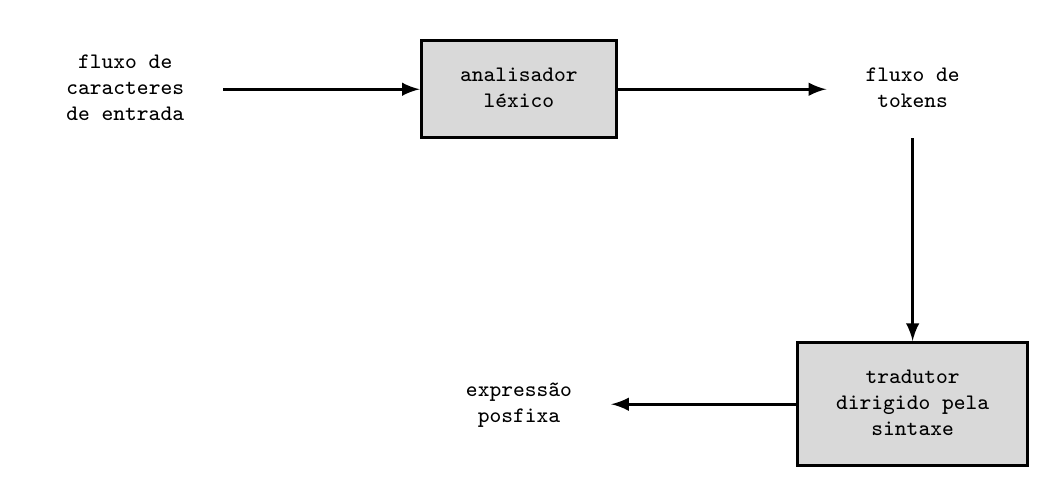
\begin{tikzpicture} 
            \node[inner sep=8pt] (A) at (0, 0) { \footnotesize \begin{tabular}{>{\tt}c}fluxo de\\ caracteres\\ de entrada\end{tabular} };
            \node[draw,fill=gray!30,very thick,inner sep=8pt] (B) at (5, 0) { \footnotesize \begin{tabular}{>{\tt}c}analisador\\ léxico\\ \end{tabular} };
            \node[inner sep=8pt] (C) at (10, 0) { \footnotesize \begin{tabular}{>{\tt}c}fluxo de\\ tokens\\ \end{tabular} };
            \node[draw,fill=gray!30,very thick,inner sep=8pt] (D) at (10, -4) { \footnotesize \begin{tabular}{>{\tt}c}tradutor\\ dirigido pela\\ sintaxe \end{tabular} };
            \node[inner sep=8pt] (E) at (5, -4) { \footnotesize \begin{tabular}{>{\tt}c}expressão\\ posfixa\\ \end{tabular} };

            \draw[-latex,very thick] (A) to (B);
            \draw[-latex,very thick] (B) to (C);
            \draw[-latex,very thick] (C) to (D);
            \draw[-latex,very thick] (D) to (E);
        \end{tikzpicture} 

    \end{figure}

\end{frame}
